\documentclass[landscape]{slides}
\usepackage{tikz}

%% set up externalization
%\usetikzlibrary{external}
%\tikzexternalize
%\tikzset{external/system call={latex \tikzexternalcheckshellescape -halt-on-error
%-interaction=batchmode -jobname "\image" "\texsource";
%dvips -o "\image".ps "\image".dvi;
%ps2eps "\image.ps"}}
%\tikzexternalize

% set up externalization
%\usetikzlibrary{external}
%\tikzset{external/system call={pdflatex \tikzexternalcheckshellescape
%                                        -halt-on-error
%                                        -interaction=batchmode
%                                        -jobname "\image" "\texsource"
%                                        && pdftops -eps "\image.pdf"}}
%\tikzexternalize[shell escape=-enable-write18]

\begin{document}
    \begin{slide}
        \begin{tikzpicture}
            \node[inner sep=0] (center) at (0,0)
            {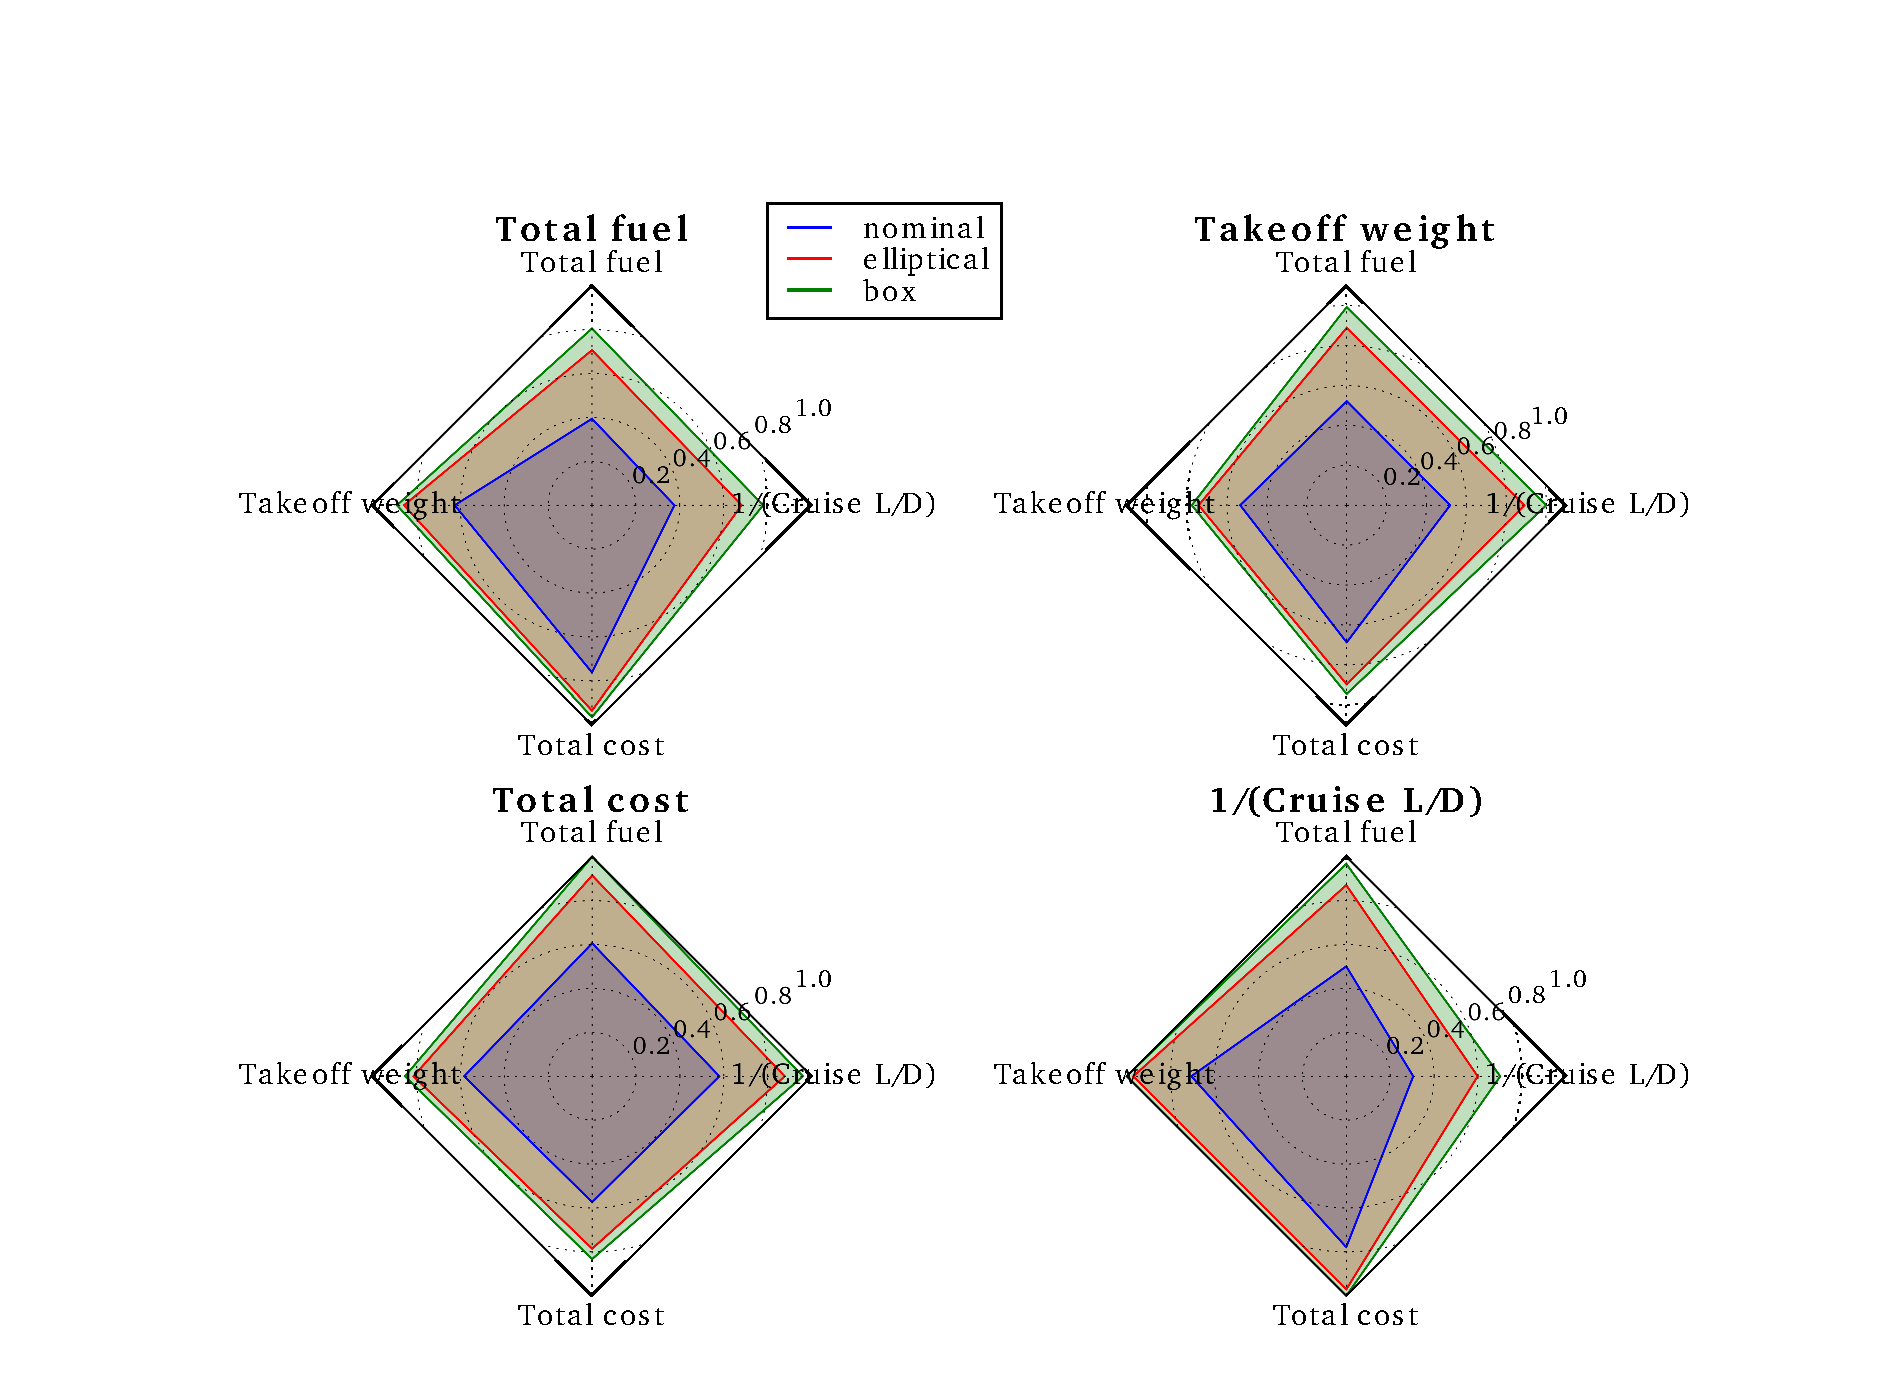
\includegraphics[trim={2cm 0 1cm 0},clip,scale=0.6]{4objradar.eps}};
            \node[inner sep=0] (ul) at (-1.0, 0.25)
            {
\includegraphics[height=3.8cm]{0nominal.eps}};
            \node[inner sep=0] (ur) at (1.0, 0.25)
            {
\includegraphics[height=3.8cm]{1nominal.eps}};
            \node[inner sep=0] (ll) at (-1.0, -2)
            {
\includegraphics[height=3.8cm]{2nominal.eps}};
            \node[inner sep=0] (lr) at (1.0, -2)
            {
\includegraphics[height=3.8cm]{3nominal.eps}};
        \end{tikzpicture}
    \end{slide}
    \begin{slide}
        \begin{figure}
            \begin{subfigure}{0.4\linewidth}
                \makebox[\textwidth]{\begin{tikzpicture}
                                         \node[inner sep=0] (l) at (-2.5,0)
                                         {
\includegraphics[trim={9.5cm 1cm 8.5cm 1cm},clip,height=3.8cm]{0nominal.eps}};
                                         \node[inner sep=0] (c) at (-1,0)
                                         {
\includegraphics[trim={9.5cm 1cm 8.5cm 1cm},clip,height=3.8cm]{0ellipsoidal.eps}};
                                         \node[inner sep=0] (r) at (.5,0)
                                         {
\includegraphics[trim={9.5cm 1cm 8.5cm 1cm},clip,height=3.8cm]{0box.eps}};
                \end{tikzpicture}}
                \caption{Total fuel}
            \end{subfigure}
            \begin{subfigure}{0.4\linewidth}
                \makebox[\textwidth]{\begin{tikzpicture}
                                         \node[inner sep=0] (l) at (-2.5,0)
                                         {
\includegraphics[trim={9.5cm 1cm 8.5cm 1cm},clip,height=3.8cm]{1nominal.eps}};
                                         \node[inner sep=0] (c) at (-1,0)
                                         {
\includegraphics[trim={9.5cm 1cm 8.5cm 1cm},clip,height=3.8cm]{1ellipsoidal.eps}};
                                         \node[inner sep=0] (r) at (.5,0)
                                         {
\includegraphics[trim={9.5cm 1cm 8.5cm 1cm},clip,height=3.8cm]{1box.eps}};
                \end{tikzpicture}}
                \caption{Takeoff weight}
            \end{subfigure}
            \begin{subfigure}{0.4\linewidth}
                \makebox[\textwidth]{\begin{tikzpicture}
                                         \node[inner sep=0] (l) at (-2.5,0)
                                         {
\includegraphics[trim={9.5cm 1cm 8.5cm 1cm},clip,height=3.8cm]{2nominal.eps}};
                                         \node[inner sep=0] (c) at (-1,0)
                                         {
\includegraphics[trim={9.5cm 1cm 8.5cm 1cm},clip,height=3.8cm]{2ellipsoidal.eps}};
                                         \node[inner sep=0] (r) at (.5,0)
                                         {
\includegraphics[trim={9.5cm 1cm 8.5cm 1cm},clip,height=3.8cm]{2box.eps}};
                \end{tikzpicture}}
                \caption{Total cost}
            \end{subfigure}
            \begin{subfigure}{0.4\linewidth}
                \makebox[\textwidth]{\begin{tikzpicture}
                                         \node[inner sep=0] (l) at (-2.5,0)
                                         {
\includegraphics[trim={9.5cm 1cm 8.5cm 1cm},clip,height=3.8cm]{3nominal.eps}};
                                         \node[inner sep=0] (c) at (-1,0)
                                         {
\includegraphics[trim={9.5cm 1cm 8.5cm 1cm},clip,height=3.8cm]{3ellipsoidal.eps}};
                                         \node[inner sep=0] (r) at (.5,0)
                                         {
\includegraphics[trim={9.5cm 1cm 8.5cm 1cm},clip,height=3.8cm]{3box.eps}};
                \end{tikzpicture}}
                \caption{1/(Cruise L/D)}
            \end{subfigure}
        \end{figure}
    \end{slide}
\end{document}
